\documentclass[11pt,a4paper]{article}

\usepackage[left=2cm,text={17cm,24cm},top=3cm]{geometry}
\usepackage[czech]{babel}
\usepackage[utf8]{inputenc}
\usepackage[T1]{fontenc}

\usepackage{url}
\usepackage{float}
\usepackage{comment}
\usepackage{etoolbox}
\usepackage{graphicx}
\usepackage{hyperref}
\usepackage{tocloft}
\usepackage{pdfpages} % include pdf

\def\UrlBreaks{\do\/\do-\do\&\do=\do\_\do?} % URL breaking characters

\newcommand{\red}[1]{\textcolor{red}{#1}} % \red{text in red}
\newcommand{\blue}[1]{\textcolor{blue}{#1}} % \blue{text in blue}
\newcommand{\TODO}{\textbf{\textcolor{red}{TODO}}} % red bold TODO
\newcommand{\tilda}{\raisebox{0.5ex}{\texttildelow}} % command \tilda for '~' character
\newcommand\ddfrac[2]{\frac{\displaystyle #1}{\displaystyle #2}}

\graphicspath{{img/}} % path to images
\patchcmd{\thebibliography}{\section*{\refname}}{}{}{} % do not create section for bibliography
\hypersetup{
    linktoc    = all,
    colorlinks = true,
    citecolor  = green,
    linkcolor  = red,
    urlcolor   = blue,
}

\begin{document}
\nocite{*}

\begin{titlepage}

    \begin{center}
        % FIX: lines must end with '%', if not then it will result in an incorrect centering
        \vfill {%
            \Huge{%
                \textsc{%
                    Fakulta informačních technologií\\[3mm]%
                    Vysoké učení technické v~Brně%
                }%
            }%
        }%

        \hfill\\[15mm]

        \begin{figure}[!h]
            \centering
            
\includegraphics[scale=0.3]{vutbr-fit-logo.eps}
        \end{figure}

        \hfill\\[10mm]

        \Huge{
            \textbf{
                MSP
            }
        }

        \hfill\\[-10mm]

        \huge{
            \textbf{
                Statistika a pravděpodobnost
            }
        }

        \hfill\\[10mm]

        \LARGE{
            \textbf{
                Semestrální projekt
            }
        }
        \vfill

    \end{center}

        \Large{
            \noindent Zpracoval: Attila Lakatos (xlakat01)\hfill \\
             Čísla zadání: 6, 15 \\
             Cvičení - skupina: čtvrtek, 09:00 \\
             Datum: \today
        }

\end{titlepage}


\newpage

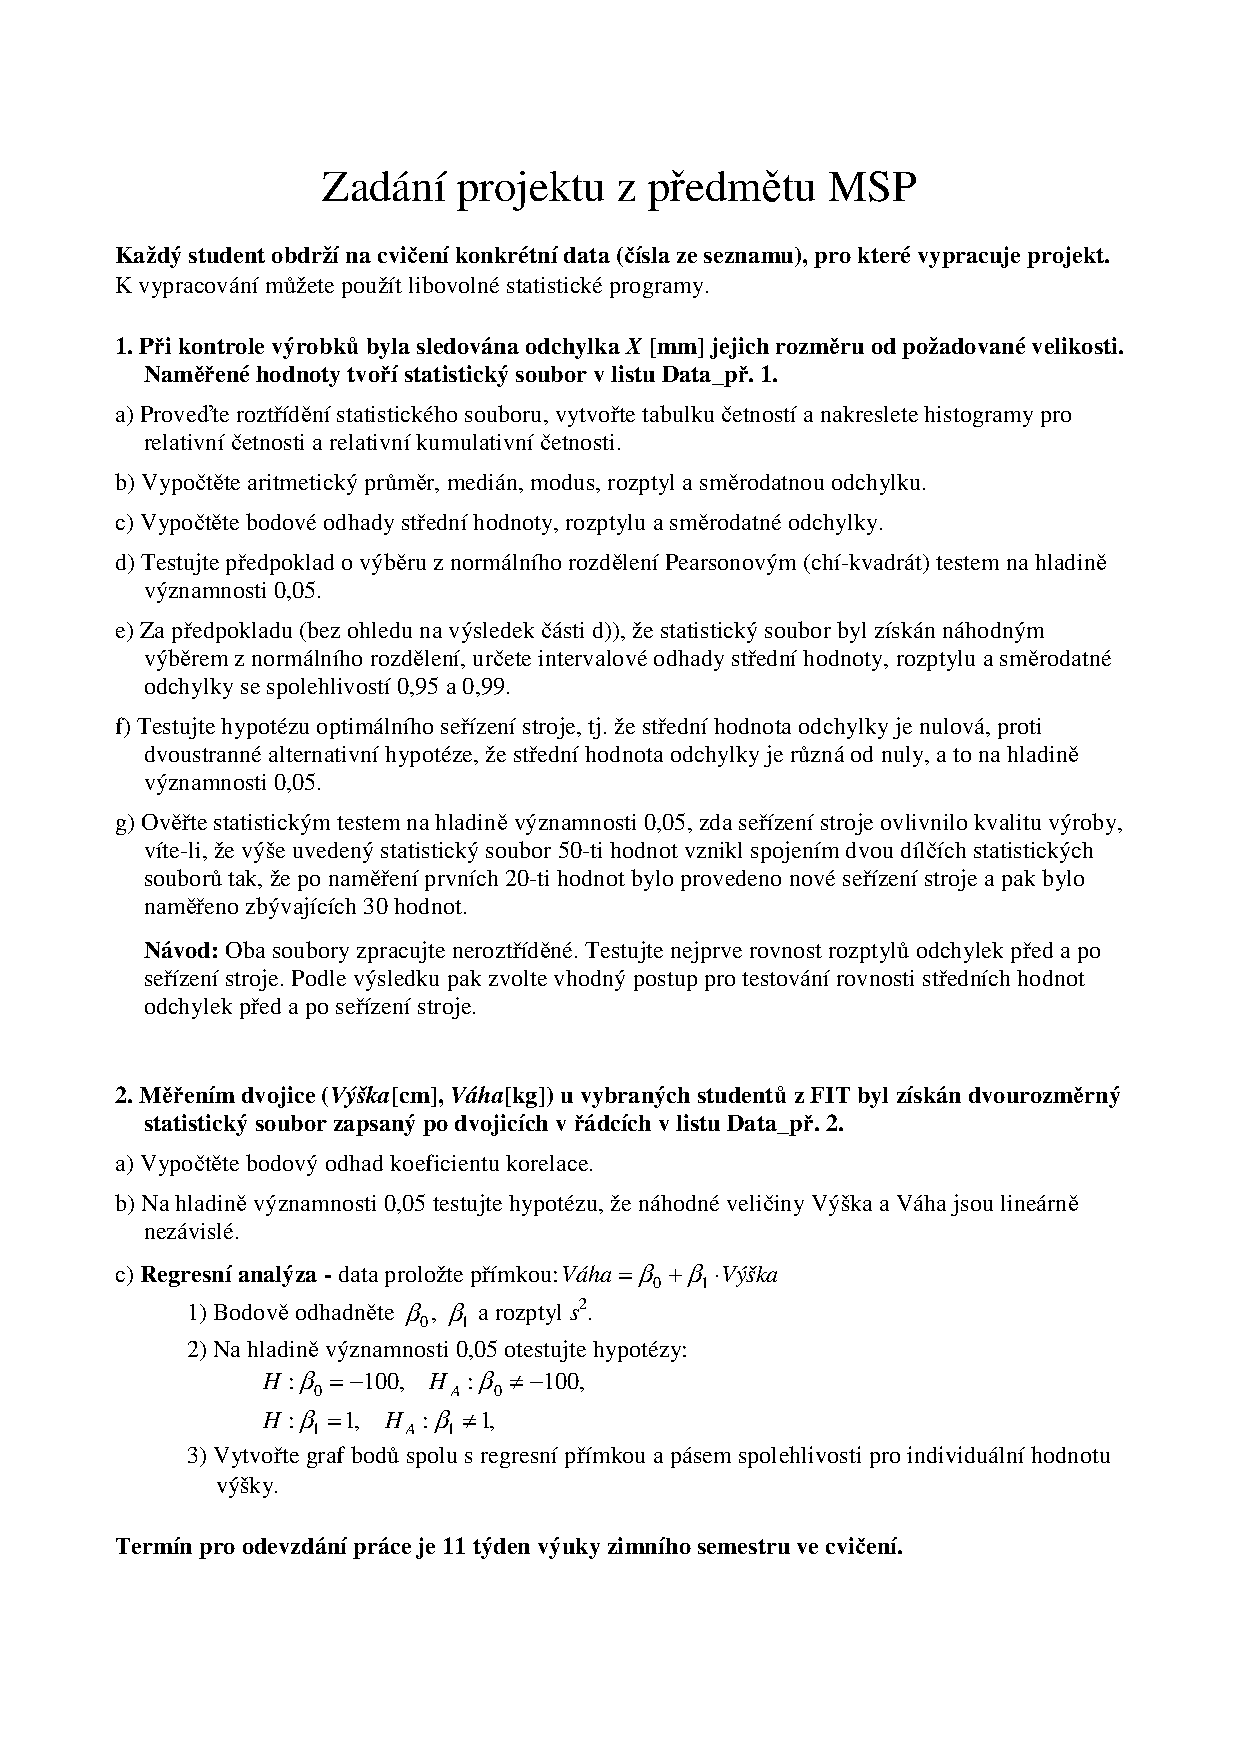
\includepdf[width=\textwidth]{img/task.pdf}

\section{Vypracování}

1. Při kontrole výrobků byla sledována odchylka X [mm] jejich rozměru od požadované velikosti. Naměřené hodnoty tvoří statistický soubor v listu Data\_př. 1.

\vspace{0,5cm}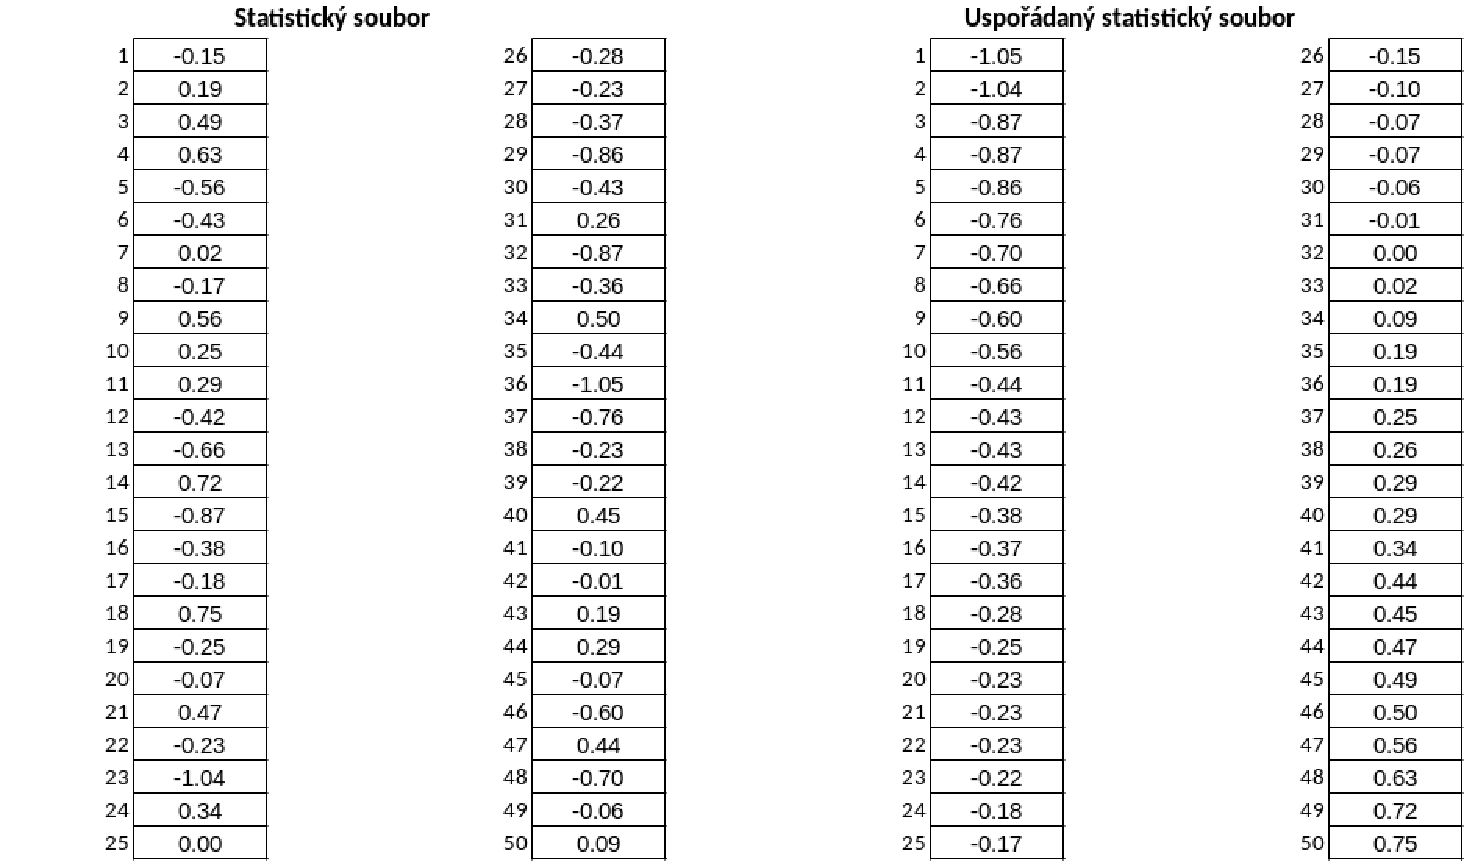
\includegraphics[width=\textwidth]{img/task1.pdf}\vspace{0,5cm}
\noindent\makebox[\linewidth]{\rule{\textwidth}{0.4pt}}
% TASK 1a

a) Proveďte roztřídění statistického souboru, vytvořte tabulku četností a nakreslete histogramy pro relativní četnosti a relativní kumulativní četnosti.
\vspace{0,5cm}

$x_{(1)} = \min\limits_i x_i = -1.05$ \\

$x_{(n)} = \max\limits_i x_i = 0.75$ \\

Variační obor: $ \langle x_{(1)}, x_{(n)} \rangle = \langle -1,05; 0,75 \rangle$ \\

Rozpětí: $ x_{(n)} - x_{(1)} = 1.8 $ \\

Počet tříd: $m = 11$ (zvoleno) \\ 

Délka třídy: $\frac{x_{(n)} - x_{(1)}}{m} = 0.163636 $

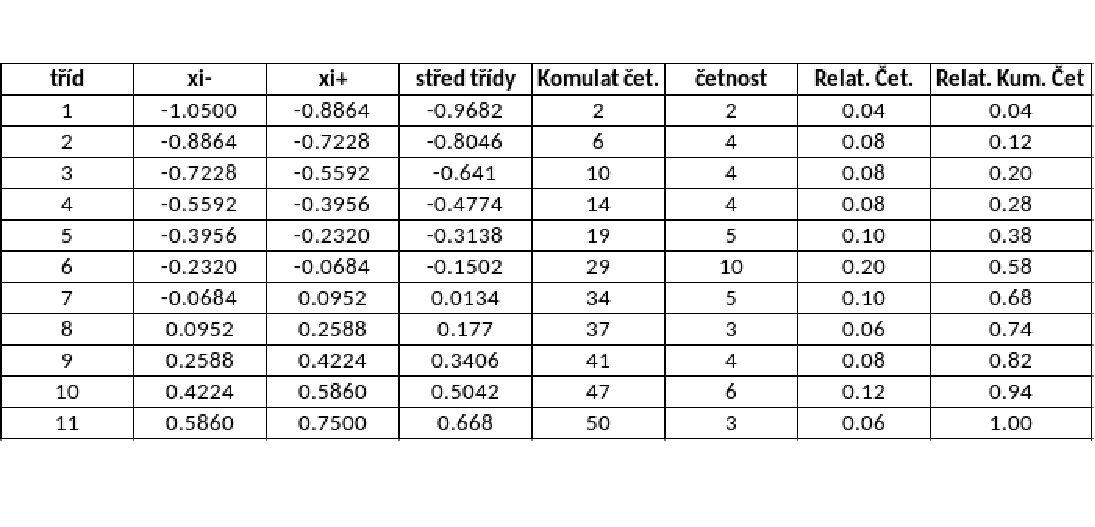
\includegraphics[width=\textwidth]{img/1atable.pdf}\vspace{-1,75cm}

\begin{figure}[H]
    \centering
    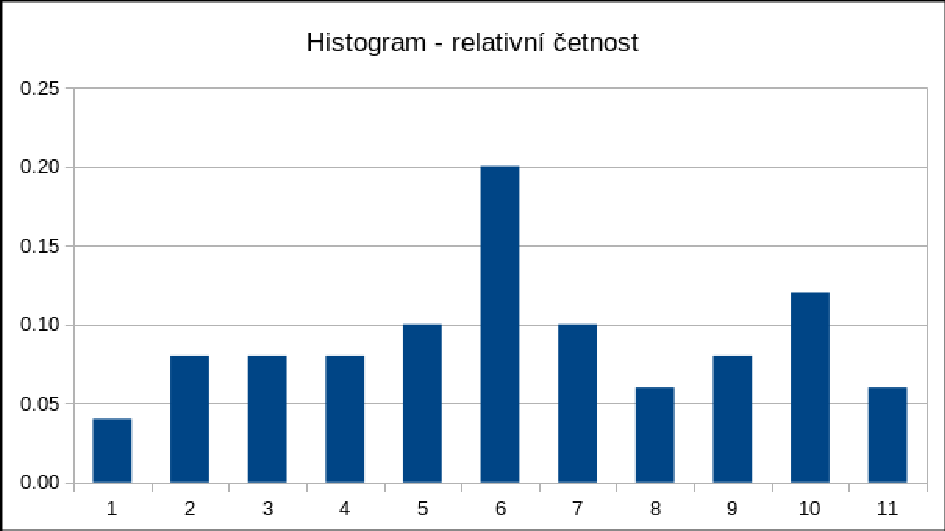
\includegraphics[width=0.55\textwidth]{img/1ahistogram1.pdf}
    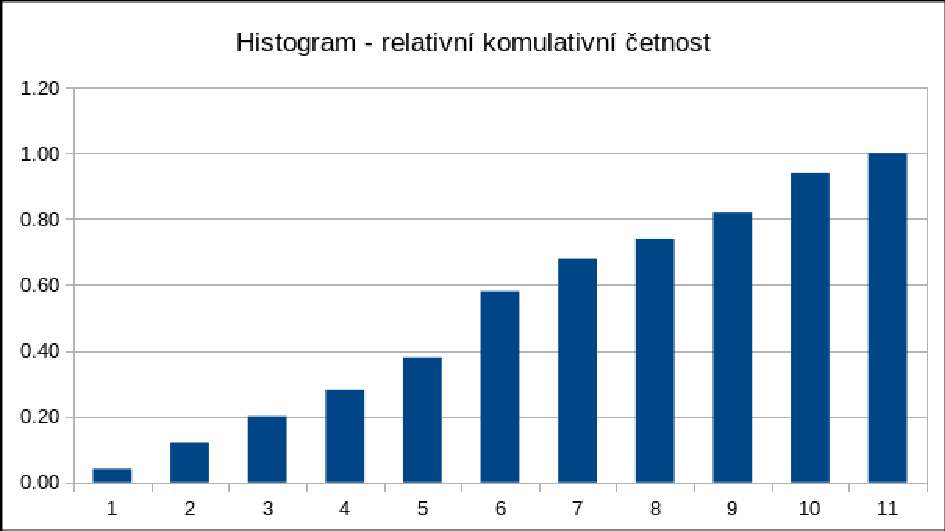
\includegraphics[width=0.55\textwidth]{img/1ahistogram2.pdf}
\end{figure}


\noindent\makebox[\linewidth]{\rule{\textwidth}{0.4pt}}
% TASK 1b

b) Vypočtěte aritmetický průměr, medián, modus, rozptyl a směrodatnou odchylku. \\

$ \overline{x} = \frac{1}{n} \sum\limits_{i=1}^n x_i = -0,1224$ \\

medián: $  \widetilde{x} = \frac{1}{2}*(-0.17 + -0.15) = 0,16 $ \\

modus: $ \widehat{x} = -0.23 (TODO) $ \\

$ s^2 = \frac{1}{n} \sum\limits_{i=1}^{n} (x_i - \overline{x})^2 = 0.21728624 $ \\

$ s = \sqrt{\frac{1}{n} \sum\limits_{i=1}^n (x_i - \overline{x})^2} = 0.466139721542801$ \\


\noindent\makebox[\linewidth]{\rule{\textwidth}{0.4pt}}
% TASK 1c

c) Vypočtěte bodové odhady střední hodnoty, rozptylu a směrodatné odchylky. \\

Bodový odhad střední hodnoty: $ \overline{x} = \frac{1}{n} \sum\limits_{i=1}^{n} x_i = -0,1224 $ \\

Bodový odhad rozptylu: $ s^2 = \frac{1}{n - 1} \sum\limits_{i=1}^{n} (x_i - \overline{x})^2 = 0.22172065306122 $ \\

Bodový odhad směrodatné odchylky: $ s = \sqrt{ \frac{1}{n - 1} \sum\limits_{i=1}^{n} (x_i - \overline{x})^2 } = 0.470872225833319 $ \\


\noindent\makebox[\linewidth]{\rule{\textwidth}{0.4pt}}
% TASK 1d

d) Testujte předpoklad o výběru z normálního rozdělení Pearsonovým (chí-kvadrát) testem na hladině významnosti 0,05. \\

\vspace{0.6cm}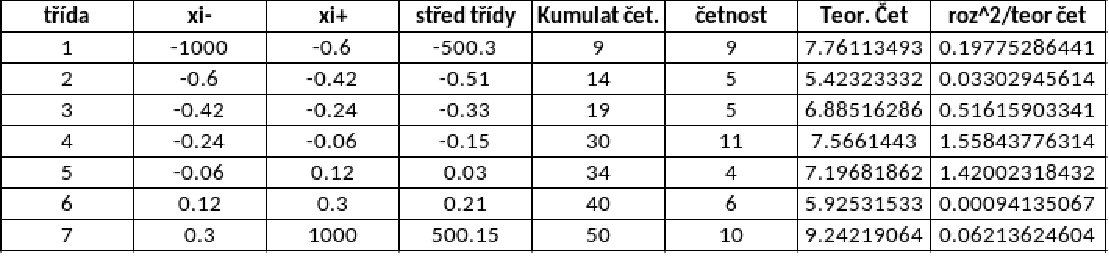
\includegraphics[width=\textwidth]{img/1dtable.pdf} \\

Testovací kritérium: $ t = \sum\limits_{j=1}^{m} \frac{(f_j - \widehat{f_j})^2}{\widehat{f_j}} = 3.788479898122$, \\

$\chi_{1-\alpha}^2$ pro $ k = 7 - 2 - 1$ stupňů volnosti: 9,488, \\

doplněk kritického oboru: $ \overline{W_{\alpha}} = \langle 0, \chi_{1-\alpha}^2 \rangle = \langle 0, 9,488 \rangle$. \\

Protože $ t \in \overline{W_{\alpha}} $, tedy hypotéza: $ X \sim N(-0,1224; 0,22172065306) $ \textbf{se nezamítá} . \\

\begin{figure}[H]
    \centering
    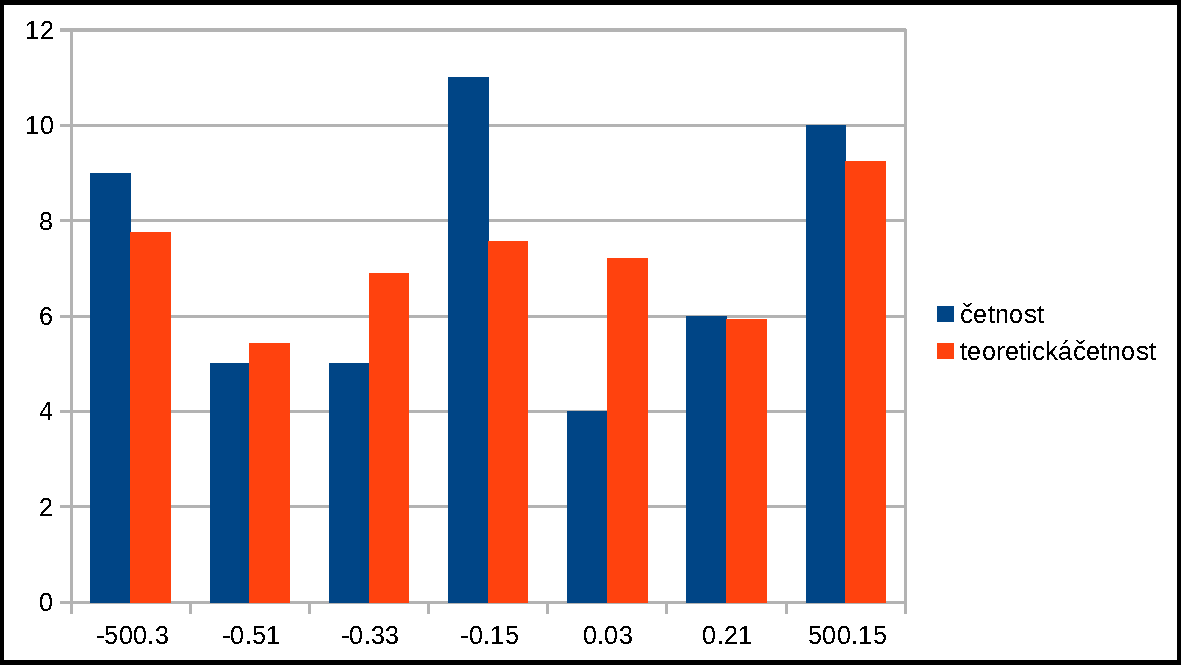
\includegraphics[width=0.75\textwidth]{img/1dhistogram.pdf}
\end{figure}

\noindent\makebox[\linewidth]{\rule{\textwidth}{0.4pt}}
% TASK 1e

e) Za předpokladu (bez ohledu na výsledek části d)), že statistický soubor byl získán náhodným výběrem z normálního rozdělení, určete intervalové odhady střední hodnoty, rozptylu a směrodatné
odchylky se spolehlivostí 0,95 a 0,99. \\

Předpoklad: $ X \sim N(\mu, \sigma^2), \sigma^2$ - neznámé \\

Bodový odhad střední hodnoty: $ \overline{x} = \frac{1}{n} \sum\limits_{i=1}^{n} x_i = -0,1224 $ \\

Bodový odhad rozptylu: $ s^2 = \frac{1}{n-1} \sum\limits{i=1}^{n} (x_i - \overline{x})^2 = 0.22172065306122 $ \\

Bodový odhad směrodatné odchylky: $ s = \sqrt{\frac{1}{n-1} \sum\limits{i=1}^{n} (x_i - \overline{x})^2} = 0.470872225833319 $ \\ 

\textbf{Intervalový odhad} parametru \textbf{$\mu:$}

0,975 kvantil Studentova rozdělení $ t_{1-\frac{\alpha}{2}} $ s $ k = n - 1 = 50 - 1 = 49 $ stupni volnosti = 2,009575237 \\

0,995 kvantil Studentova rozdělení $ t_{1-\frac{\alpha}{2}} $ s $ k = n - 1 = 50 - 1 = 49 $ stupni volnosti = 2,6779951964 \\

$ \alpha = 0,05 : \biggl< \overline{x} - t_{1-\alpha/2} \frac{s}{\sqrt{n}} ; \overline{x} + t_{1-\alpha/2} \frac{s}{\sqrt{n}} \biggr> = \Bigl< -0,256220406; 0,011420406 \Bigr>$ \\

$ \alpha = 0,01 : \biggl< \overline{x} - t_{1-\alpha/2} \frac{s}{\sqrt{n}} ; \overline{x} + t_{1-\alpha/2} \frac{s}{\sqrt{n}} \biggr> = \Bigl< -0.300731419; 0.055931419 \Bigr>$ \\

\vspace{0,7cm}
\textbf{Intervalový odhad} parametru \textbf{$\sigma^2:$}

0,975 kvantil Pearsova rozdělení $ \chi_{\alpha/2}^2 $ s $ k = n - 1 = 50 - 1 = 49 $ stupni volnosti $ = 31,55491646 $ \\

0,975 kvantil Pearsova rozdělení $ \chi_{1-\alpha/2}^2 $ s $ k = n - 1 = 50 - 1 = 49 $ stupni volnosti $ = 70,22241357 $ \\

0,995 kvantil Pearsova rozdělení $ \chi_{\alpha/2}^2 $ s $ k = n - 1 = 50 - 1 = 49 $ stupni volnosti $ = 27,24934921 $ \\

0,995 kvantil Pearsova rozdělení $ \chi_{1-\alpha/2}^2 $ s $ k = n - 1 = 50 - 1 = 49 $ stupni volnosti $ = 78,23070806 $ \\

$ \alpha = 0,05 : \biggl< \frac{(n - 1) s^2}{\chi_{1-\alpha/2}^2} ; \frac{(n - 1) s^2}{\chi_{\alpha/2}^2} \biggr> = \Bigl< 0.154712882 ; 0.344298551 \Bigr> $ \\

$ \alpha = 0,01 : \biggl< \frac{(n - 1) s^2}{\chi_{1-\alpha/2}^2} ; \frac{(n - 1) s^2}{\chi_{\alpha/2}^2} \biggr> = \Bigl< 0.138875287 ; 0.39869987 \Bigr> $ \\

\vspace{0,7cm}
\textbf{Intervalový odhad} parametru \textbf{$\sigma:$}

$ \alpha = 0,05 : \biggl< \sqrt{\frac{(n - 1) s^2}{\chi_{1-\alpha/2}^2}} ; \sqrt{\frac{(n - 1) s^2}{\chi_{\alpha/2}^2}} \biggr> = \Bigl< \sqrt{0.154712882} ; \sqrt{0.344298551} \Bigr> = \Bigl< 0.393335584  ; 0.586769589 \Bigr> $ \\

$ \alpha = 0,01 : \biggl< \sqrt{\frac{(n - 1) s^2}{\chi_{1-\alpha/2}^2}} ; \sqrt{\frac{(n - 1) s^2}{\chi_{\alpha/2}^2}} \biggr> = \Bigl< \sqrt{0.138875287} ; \sqrt{0.39869987} \Bigr> = \Bigl< 0.372659747 ; 0.631426852 \Bigr> $ \\

\noindent\makebox[\linewidth]{\rule{\textwidth}{0.4pt}}
\newpage

% TASK 1f
f) Testujte hypotézu optimálního seřízení stroje, tj. že střední hodnota odchylky je nulová, proti dvoustranné alternativní hypotéze, že střední hodnota odchylky je různá od nuly, a to na hladině významnosti 0,05. \\

\textbf{Studentův jednovýběrový test:} \\

\textbf{Testujeme hypotézu} $ H_0 : \mu = 0: $ \\

testovací kritérium: $ t = \frac{\overline{x} - \mu_0}{s} \sqrt{n} = \frac{\overline{x} - 0}{s} \sqrt{n} = -1.838075496$ \\

doplněk kritického oboru: $ \overline{W_\alpha} = \Bigl< -t_{1-alpha/2} , t_{1-\alpha/2} \Bigr> $ pro alternativní hypotézu: $ H_A : \mu \ne \mu_0, 0,975 $ kvantil Studentova rozdělení $ t_{1-\alpha/2} $ s $ k = n - 1 = 50 - 1 = 49 $ stupni volnosti $ = 2,009575237 $ \\

$ \overline{W_\alpha} = \Bigl< -t_{1-\alpha/2} , t_{1-\alpha/2} \Bigr> = \Bigl< -2,009575237, 2,0095752 \Bigr> $

Protože $ t \in \overline{W_\alpha} $, tak hypotéza $ H_0 : \mu = 0 $ \textbf{se nezamítá} a alternativní hypotéza $ H_A : \mu \ne 0 $ se zamítá.

\noindent\makebox[\linewidth]{\rule{\textwidth}{0.4pt}}

% TASK 1g

g) Ověřte statistickým testem na hladině významnosti 0,05, zda seřízení stroje ovlivnilo kvalitu výroby,
víte-li, že výše uvedený statistický soubor 50-ti hodnot vznikl spojením dvou dílčích statistických
souborů tak, že po naměření prvních 20-ti hodnot bylo provedeno nové seřízení stroje a pak bylo
naměřeno zbývajících 30 hodnot.


\begin{figure}[H]
    \centering
    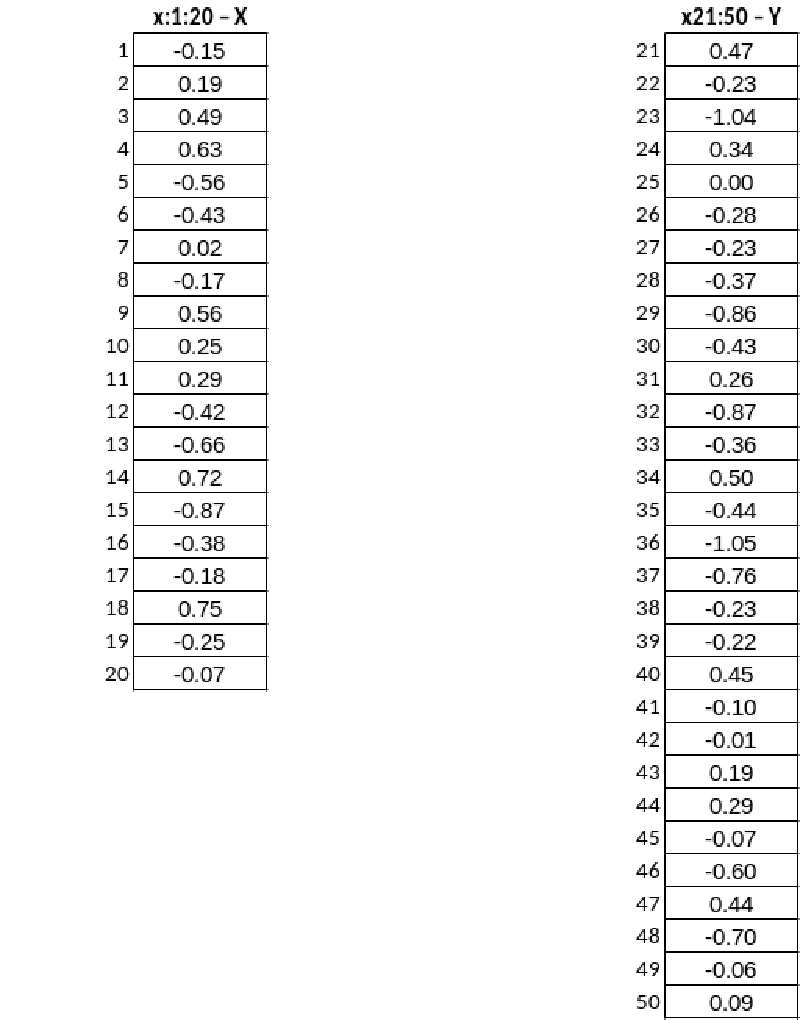
\includegraphics[width=0.60\textwidth]{img/1gtable.pdf}
\end{figure}

\begin{table}[]
    \centering
    \begin{tabular}{|c|c|c|}
    \hline
                                     & X                               & Y                               \\ \hline
    n                                & 20                              & 30                              \\ \hline
    průměr                           & -0,012                          & -0,196                          \\ \hline
    rozptyl s\textasciicircum{}2     & 0,218736                        & 0,20277733                      \\ \hline
    \multicolumn{1}{|l|}{směr\_odch} & \multicolumn{1}{l|}{0,46769221} & \multicolumn{1}{l|}{0,45030804} \\ \hline
    \end{tabular}
\end{table}

\textbf{Test rovnosti rozptylů – F-test:} \\

\textbf{Testujeme hypotézu} $H_0 : \sigma_{X}^2 = \sigma_{Y}^2 : $\\

testovací kritérium: $ t = \frac{s^2(X)}{s^2(Y)} = \frac{0,218736}{0,20277733} = 1.078700464 $ \\

doplněk kritického oboru: $ \overline{W_\alpha} = \Bigl< F_{\alpha/2} (n - 1, m - 1), F_{1-\alpha/2} (n - 1, m - 1) \Bigr> $ pro $ H_A : \sigma_{X}^2 \ne \sigma_{Y}^2$, $F_{\alpha/2}(k_1, k_2), F_{1-\alpha/2}(k_{1}, k_2) $ jsou kvantily Fischerova-Snedecorova rozdělení s $ k_1 = n - 1 $ a $ k2 = m - 1 $ stupni volnosti. \\

$ F_{\alpha/2}(19, 29) = 0,416329667 $ \\

$ F_{1-\alpha/2}(19, 29) = 2,231274 $ \\

$ \Bigl< F_{\alpha/2} (n - 1, m - 1), F_{1-\alpha/2} (n - 1, m - 1) \Bigr> = \Bigl< 0,416329667, 2,231274 \Bigr> $ \\

Protože $ t \in \overline{W_\alpha}$, tedy hypotéza $ H_0 : \sigma_{X}^2 = \sigma_{Y}^2$ \textbf{se nezamítá}. \\

\vspace{0,7cm}
\textbf{Studentův dvouvýběrový test:} \\
 
\textbf{Testujeme hypotézu} $ H_0 : \mu_X - \mu_Y $ \textbf{za podmínky} $ \sigma_{X}^2 = \sigma{Y}^2 $\\

testovací kritérium: $ t = \ddfrac{\overline{x} - \overline{y} - \mu_0}{\sqrt{(n - 1) s^2(X) + (m - 1) s^2(Y)} } \sqrt{ \ddfrac{n * m(n + m - 2)}{n + m} } = 1.393918382 $ \\

doplněk kritického oboru: $ \overline{W_\alpha} = \Bigl< -t_{1-\alpha/2}, t_{1-\alpha/2} $ pro $ H_A : \mu_X - \mu_Y \ne 0 $, \\

$ t_{1-\alpha/2} $ - kvantil Studentova rozdělení s $ k = n + m - 2 = 20 + 30 - 2 = 48 $ stupni volnosti. \\

$ t_{1-\alpha/2} = 2,010634758 $ \\

$ \overline{W_\alpha} = \Bigl< -t_{1-\alpha/2}, t_{1-\alpha/2} \Bigr> = \Bigl< -2,010634758; 2,010634758 \Bigr> $ \\

Protože $ t \in \overline{W_\alpha} ,$ tedy hypotéza: $ H_0 : \mu_X - \mu_Y = 0 $ \textbf{se nezamítá}.

\newpage


% TASK 2
\textbf{2. Měřením dvojice (Výška[cm], Váha[kg]) u vybraných studentů z FIT byl získán dvourozměrný
statistický soubor zapsaný po dvojicích v řádcích v listu Data\_př. 2.}

\begin{figure}[H]
    \centering
    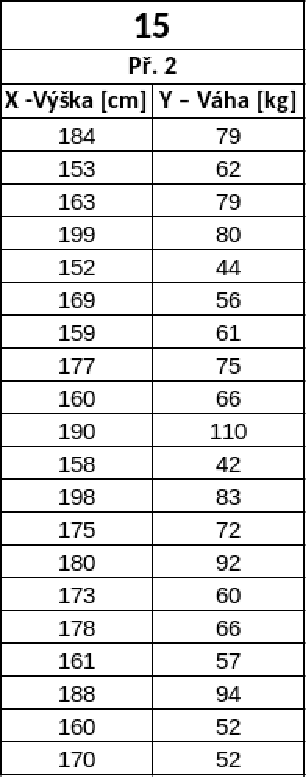
\includegraphics[scale=0.85]{img/2table.pdf}
\end{figure}

$ n = 20 $ \\

$ \overline{x} = 172,35 $ \\

$ \overline{y} = 69,172607489 $ \\

$ \sum\limits_{i=1}^{n} x_{i}^2 = 597981 $ \\

$ \sum\limits_{i=1}^{n} y_{i}^2 = 101528,70165 $ \\

$ \sum\limits_{i=1}^{n} x_i y_i = 242013,65983 $ \\

\noindent\makebox[\linewidth]{\rule{\textwidth}{0.4pt}}

% TASK 2a
a) Vypočtěte bodový odhad koeficientu korelace. \\

$ r = \ddfrac{\sum\limits_{i=1}^{n} x_i y_i - n * \overline{x} * \overline{y}}{\sqrt{\biggl( \sum\limits_{i=1}^{n} x_{i}^2 - n * \overline{x}^2 \biggr) \biggl( \sum\limits_{i=1}^n x_{i}^2 - n * \overline{y}^2 \biggr) } }  = 0,7506810259 $ \\

\noindent\makebox[\linewidth]{\rule{\textwidth}{0.4pt}}

%TASK 2b
b) Na hladině významnosti 0,05 testujte hypotézu, že náhodné veličiny Výška a Váha jsou lineárně
nezávislé.

Testujeme hypotézu $ H_0 : \rho = 0 : $ \\

testovací kritérium: $ t = \ddfrac{|r|\sqrt{n - 2}}{\sqrt{1 - r^2}} = 4,8207045282 $ \\

doplněk kritického oboru: $ \overline{W_\alpha} = \Bigl< 0, t_{1-\alpha/2} \Bigr> $ pro alternativní hypotézu: $ H_A : \rho \ne 0, $ \\

$ t_{1-\alpha/2}(n - 2) = t_{0,975} (20 - 2) = 2,100922037 $ \\

Protože $ t \notin \overline{W_\alpha} $, tedy hypotéza: $ H_0 : \rho = 0 $ \textbf{se zamítá}. \\

\noindent\makebox[\linewidth]{\rule{\textwidth}{0.4pt}}

%TASK 2c
c) \textbf{Regresní analýza} - data proložte přímkou: Váha $= \beta_0 + \beta_1 * $ Výška \\

\begin{figure}[H]
    \centering
    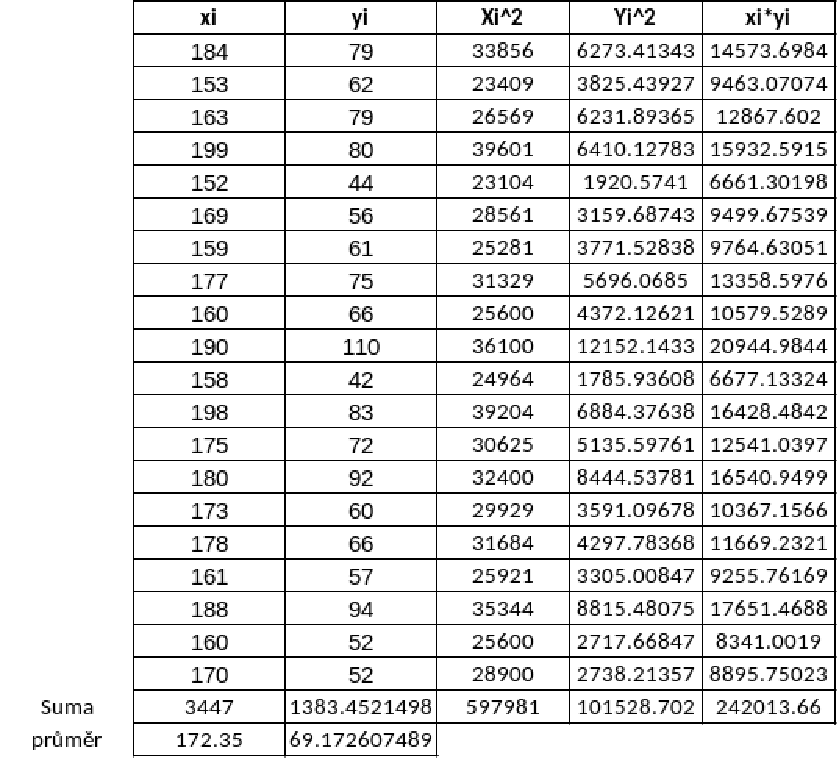
\includegraphics[width=0.70\textwidth]{img/1ctable.pdf}
\end{figure}

Tedy: \\

$ n = 20,$ \\

$\sum\limits_{i=1}^n x_i = 3447, \sum\limits_{i=1}^n y_i = 1383,4521498, $ \\

$\sum\limits_{i=1}^{n} x_{i}^2 = 597981, \sum\limits_{i=1}^n y_{i}^2 = 101528,702, $ \\

$\sum\limits_{i=1}^n x_i * y_i = 242013,66. $

\newpage

$ det(H) = n \sum\limits_{i=1}^{n} x{i}^2 - \Bigl( \sum\limits_{i=1}^{n} x_i \Bigr)^2 = 77811$ \\

%TASK 2c SUBTASK 1
1) Bodově odhadněte $ \beta_0, \beta_1 $ a rozptyl $ s^2 $. \\

$ b_2 = \ddfrac{1}{det(h)} \biggl( n \sum\limits_{i=1}^{n} x_i y_i - \sum\limits_{i=1}^{n} x_i \sum\limits_{i=1}^{n} y_i \biggr) = 0,9190684646 $ \\

$ b_1 = \overline{y} - b_2 * \overline{x} = -89,22884239 $ \\

$ y = b_1 + b_2 * x = -89,22884239 + 0,9190684646 $ \\

$ S_{min}^{*} = \sum\limits_{i=1}^{n} y_{i}^2 - b_1 \sum\limits_{i=1}^n y_i - b_2 \sum\limits_{i=1}^n x_i y_i = 2545,4127125 $ \\

$ s^2 = \ddfrac{S_{min}^{*}}{n - 2} = \ddfrac{S_{min}^{*}}{20 - 2} = 141,41181736 $ \\
\vspace{0,7cm}

%TASK 2c SUBTASK 2
2) Na hladin ě významnosti 0,05 otestujte hypotézy: \\

$ H : \beta_0 = -100, H_A : \beta_0 \ne -100 $, \\

$ h^{11} = \ddfrac{\sum\limits_{i=1}^{n} x_{i}^2}{det(H)} = 7,68504453097891 $ \\

$ t = \ddfrac{b_1 - (-100)}{s\sqrt{h^{11}}} = 0,326735508653823 $ \\

$ t_{1-\alpha/2} (n - 2) = t_{0,975} (20 - 2) = 2,100922037 $ \\

$ t \in \overline{W} = \Bigl< -2,100922037, 2,100922037 \Bigr> $, a tedy $ H : \beta_1 = -100 $ \textbf{se nezamítá} \\

$ H: \beta_1 = 1, H_A : \beta_1 \ne 1, $ \\

$ h_{22} = \ddfrac{n}{det(H)} = 0.000257033067304 $ \\

$ t = \ddfrac{b_2 - 1}{s * \sqrt{h^22}} = -0.424502672132561 $ \\

$ t_{1-\alpha/2} (n - 2) = t_{0,975} (20 - 2) = 2,100922037 $ \\

$ t \in \overline{W} = \Bigl< -2,100922037, 2,100922037 \Bigr>, $ a tedy $ H : \beta_2 = 1 $ \textbf{se nezamítá} \\

\noindent\makebox[\linewidth]{\rule{\textwidth}{0.4pt}}
\newpage








\section{Literatura}
\bibliographystyle{czechiso}
\begin{flushleft}
    \bibliography{quotation}
\end{flushleft}

\end{document}
